\chapter{实验结果与分析}
\label {exp}
本章主要介绍如何对补丁兼容性检测工具进行实验,并给出了实验结果和分析。

\section{实验设计}
\label {exp_des}

考虑到本文讨论的软件补丁兼容性检测问题是一个工业界中常见的问题,广泛存在于各类项目的开发、维护过程中,因此在对该检测工具进行实验时,应当选择工业界中常见、常用的中大型项目,使得实验结果具有较强的说服力,能够说明本文所提出的检测方法是否能切实解决工业界中面对的实际问题。

可见,实验应当具备如下目的:
\begin{itemize}
	\item 测试检测工具是否能够对中大型项目成功进行分析。该项可以说明本文方法的可用性,即是否能够对工业界的实际项目进行分析。
	\item 测试检测工具是否能够找到补丁的兼容性问题,其检测结果是否正确。该项可以说明本文方法的正确性,即是否能够正确地检测到的补丁间的语义冲突。
	\item 测试检测工具能找到多少兼容性问题。该项可以说明本文方法的实用性,即是否能够完全覆盖所有的补丁间冲突。
\end{itemize}

因此,本章中应当进行满足上述要求的实验,并对其结果给出相应的量化表述。

根据上面的需求,本章中的实验过程可以设计如图\ref {des_exp}所示。

\begin{figure}[H]
	\centering
	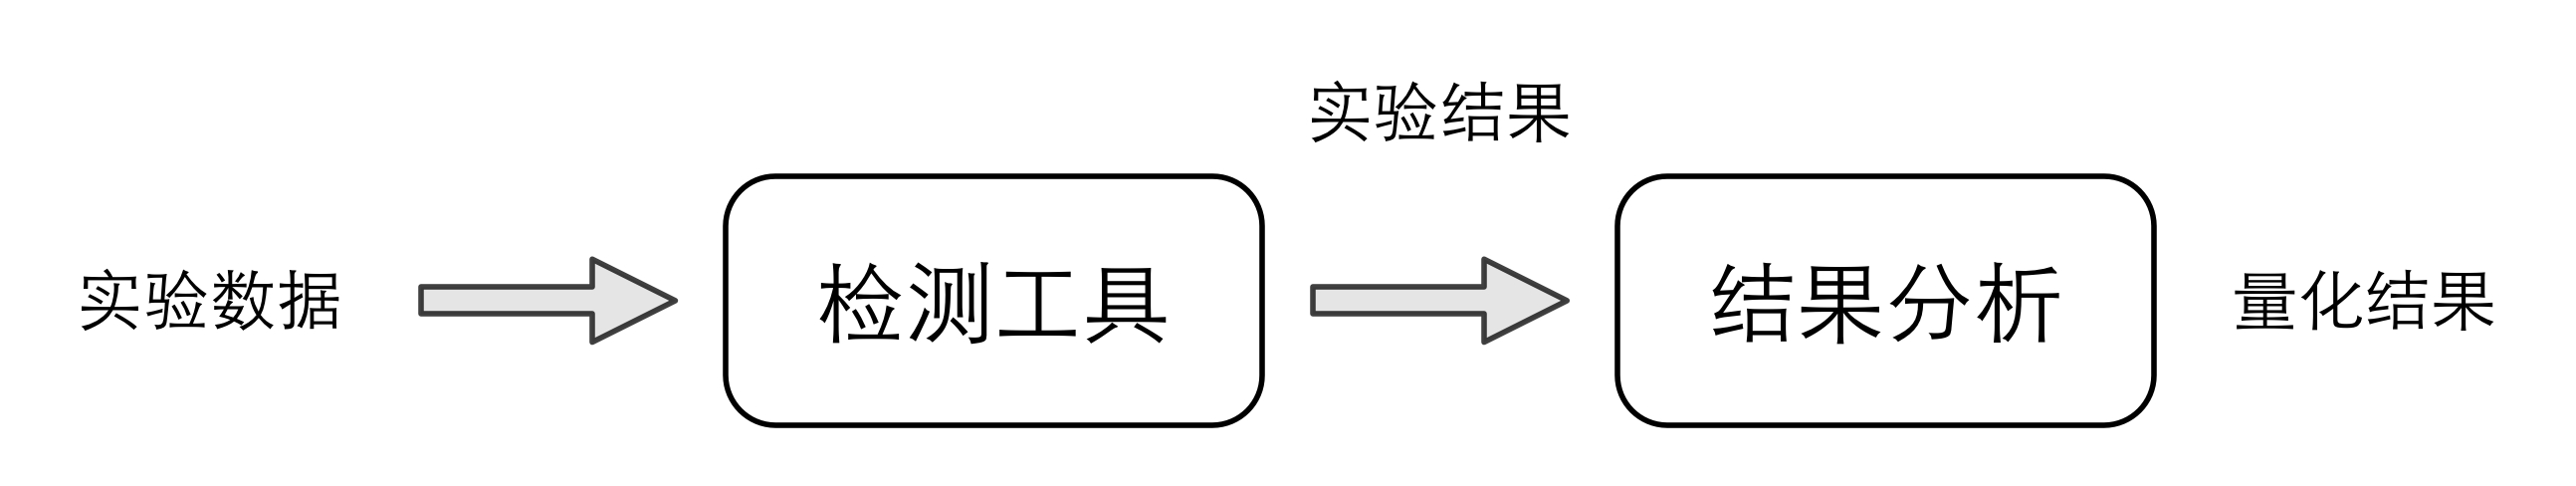
\includegraphics[width=.8\columnwidth]{chap07_exp}
	\caption {实验设计}
	\label {des_exp}	
\end{figure}


下面就本文中所采用的实验平台,对其配置说明如下:
\begin{itemize}
	\item 操作系统:Mac OS X 10.9
	\item CPU:2.4 GHz Intel Core i5
	\item 内存:8 GB 1600 MHz DDR3
	\item 硬盘:251 GB APPLE SSD SM0256F Media
\end{itemize}

\section{实验案例}
\label {exp_data}

本文将采用Eclipse JDT Core项目和其相关的补丁作为实验案例,以测试检测工具的可靠性和可用性等。JDT Core是Eclipse工具的基础组件,用于支持Java语言的编译等功能。该项目的相关信息可以参见表\ref {jdt_core}。

\begin{table}[H]
	\caption{Eclipse JDT Core}
	\label{jdt_core}
	\centering
	\begin{tabular}{llc}
		\toprule[1.5pt]
		{\heiti 信息} & {\heiti 描述} \\\midrule[1pt]
		语言 & Java \\
		文件数 & 约1200个\\
		代码量 & 约45W行\\
		\bottomrule[1.5pt]
	\end{tabular}
\end{table}

Groovy-Eclipse是一个Eclipse插件集合,用于为Groovy语言提供Eclipse的工具支持。通过Groovy-Eclipse提供的Eclipse JDT Core功能增强补丁,Groovy语言的代码可以被Eclipse JDT Core编译为Java字节码,从而在JVM上运行。这一特性使得Groovy可以调用其他Java语言编写的库,从而大大提升了其可用性。本文选择应用该功能增强补丁后的Eclipse JDT Core作为实验中版本$v_3$的来源。

Eclipse JDT Core项目截止目前已推出至发行版4.4.2,本文从中选择了若干个发行版作为实验中版本$v_1$和$v_2$的来源。实验数据的具体选择可以参考表\ref {exp_data},对各版本的具体说明可以参考表\ref {exp_version}。由于版本$v_4$是由版本合并而来,因此在表\ref {exp_data}中不予列出。

根据表\ref {exp_data},本文共选择了7个发行版本作为版本$v_2$的来源。也就是说,实验将以固定的版本$v_1$和$v_3$为基准,并选择不同的实验数据作为版本$v_2$来进行实验。

%这样做的好处是可以对本文中所提出的补丁兼容性检测工具进行详尽的测试,包括:
%\begin{itemize}
%	\item 测试该工具能否针对工业界实际项目进行分析。
%	\item 测试该工具能否切实贴合工业界的实际需求。
%	\item 测试该工具能否对同一软件系统的多个不同版本具有普遍适用性。
%\end{itemize}

\begin{table}[H]
	\caption{实验数据}
	\label{exp_data}
	\centering
	\begin{tabular}{llc}
		\toprule[1.5pt]
		{\heiti 代码} & {\heiti 发行版本} & {\heiti 版本对照} \\\midrule[1pt]
		Eclipse JDT Core & 4.3.2 & $v_1$ \\
		Groovy-Eclipse JDT Core & 4.3.2 & $v_3$\\
		Eclipse JDT Core & 4.4 & $v_2$\\
		Eclipse JDT Core & 4.4.2 & $v_2$\\
		Eclipse JDT Core & 4.3 & $v_2$\\
		Eclipse JDT Core & 4.3.1 & $v_2$\\
		Eclipse JDT Core & 4.2 & $v_2$\\
		Eclipse JDT Core & 4.2.1 & $v_2$\\
		Eclipse JDT Core & 4.2.2 & $v_2$\\
		\bottomrule[1.5pt]
	\end{tabular}
\end{table}

\begin{table}
	\caption{版本对照表}
	\label{exp_version}
	\centering
	\begin{tabular}{llc}
		\toprule[1.5pt]
		{\heiti 版本} & {\heiti 描述} \\\midrule[1pt]
		$v_1$ & 旧版本 \\
		$v_2$ & 新版本\\
		$v_3$ & 应用补丁p后的旧版本\\
		$v_4$ & 版本$v_2$和版本$v_3$合并后版本,相当于应用补丁p后的新版本\\
		\bottomrule[1.5pt]
	\end{tabular}
\end{table}

\section{实验结果与分析}
\label {exp_result}

由于检测方法由多个步骤组成,因此实验是分步进行的,本节将给出每个步骤的输入输出数据,并对其结果加以分析。

\subsection{版本迁移}

如章节\ref {sec_method}所述,实验首先需要完成将补丁p应用于版本$v_2$的过程。该过程采用git工具进行版本合并,并使用Beyond Compare工具解决合并时可能出现的语法冲突。

根据上节中所选择的实验案例,补丁的版本迁移过程可以参考图\ref {exp_git_merge}。该过程以Eclipse JDT Core发行版4.3.2作为旧版本$v_1$,以Groovy-Eclipse JDT Core发行版4.3.2作为版本$v_3$,以其他Eclipse JDT Core发行版作为版本$v_2$,并为不同的版本$v_2$创建了独立分支,用于实现各自的版本合并过程。

版本合并过程中检测到的待解决冲突数量可以参见表\ref {data_git_merge}。通过Beyond Compare工具,这些冲突都能够得到解决。

根据图\ref {data_merge_compile}可以发现,冲突最少的是版本4.3.x,几乎为0\%,这可能是由于版本4.3到版本4.3.2的升级过程改动较少而造成的。而对于版本4.4.x来说,冲突百分比甚至高达20\%至30\%,这可能是由于版本升级较大的缘故。
%根据实验结果,这些冲突95\%以上都可以采用Beyond Compare工具中推荐的方案进行解决,只有极少部分代码需要进行手工解决。




\begin{table}[H]
	\caption{版本合并结果}
	\label{data_git_merge}
	\centering
	\begin{tabular}{llcc}
		\toprule[1.5pt]
		{\heiti 代码} & {\heiti 发行版本} & {\heiti 冲突文件数量} & {\heiti 所有文件}\\\midrule[1pt]
		Eclipse JDT Core & 4.4 & 313 & 1285\\
		Eclipse JDT Core & 4.4.2 & 596 & 1281\\
		Eclipse JDT Core & 4.3 & 10 & 1209\\
		Eclipse JDT Core & 4.3.1 & 10 & 1209\\
		Eclipse JDT Core & 4.2 & 50 & 1205\\
		Eclipse JDT Core & 4.2.1 & 49 & 1205\\
		Eclipse JDT Core & 4.2.2 & 49 & 1205\\
		\bottomrule[1.5pt]
	\end{tabular}
\end{table}

\begin{figure}[H]
	\centering
	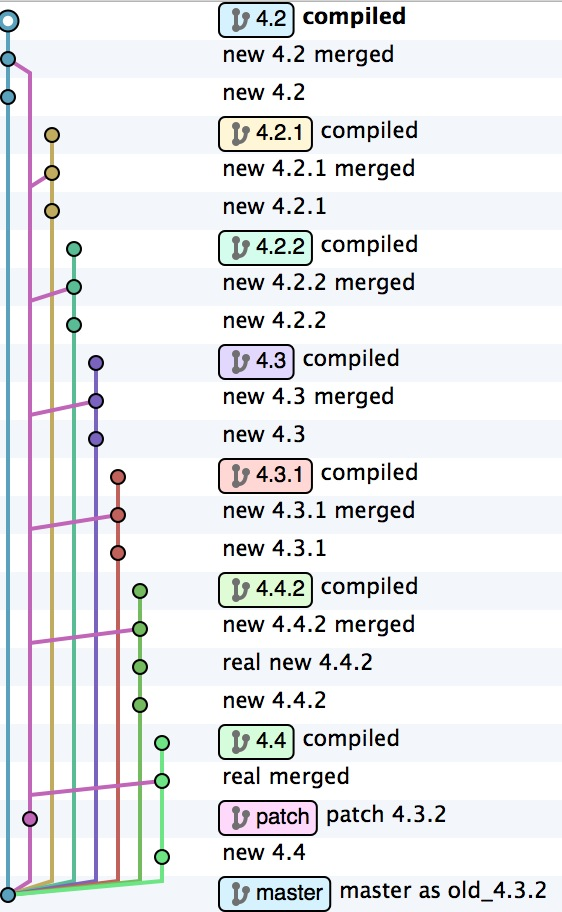
\includegraphics[height=.8\columnwidth]{chap07_git_merge}
	\caption {git版本合并}
	\label {exp_git_merge}	
\end{figure}

%\begin{figure}[H]
%	\centering
%	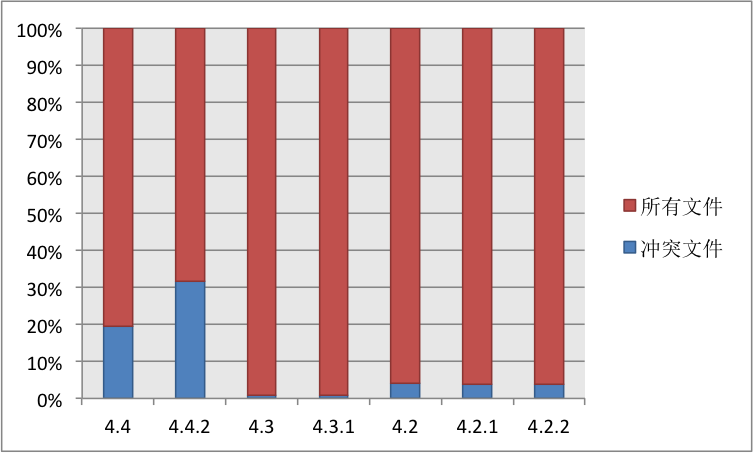
\includegraphics[width=.6\columnwidth]{merge1}
%	\caption {版本合并结果}
%	\label {data_merge}	
%\end{figure}


在实验过程中,由于后续的影响域分析模块需要提供Java代码编译后产生的Class文件,合并后的版本$v_4$还需要编译。实验结果表明,绝大多数的文件都能够正常编译通过,只有极少部分文件由于合并出错等原因而无法编译通过。该部分数据可以参考表\ref {data_git_merge2}。同样,从图\ref {data_merge_compile}可以看出,编译失败的文件数量所占的百分比很低。


参考图\ref {data_merge_compile},对比编译过程中的失败数据与版本合并中的冲突数据,可见二者的变化过程是较为吻合的。

\begin{table}[H]
	\caption{编译结果}
	\label{data_git_merge2}
	\centering
	\begin{tabular}{llcc}
		\toprule[1.5pt]
		{\heiti 代码} & {\heiti 发行版本} & {\heiti 编译失败文件} & {\heiti 所有文件}\\\midrule[1pt]
		Eclipse JDT Core & 4.4 & 23 & 1285\\
		Eclipse JDT Core & 4.4.2 & 18 & 1281\\
		Eclipse JDT Core & 4.3 & 0 & 1209\\
		Eclipse JDT Core & 4.3.1 & 1 & 1209\\
		Eclipse JDT Core & 4.2 & 4 & 1205\\
		Eclipse JDT Core & 4.2.1 & 4 & 1205\\
		Eclipse JDT Core & 4.2.2 & 1 & 1205\\
		\bottomrule[1.5pt]
	\end{tabular}
\end{table}

%\begin{figure}[H]
%	\centering
%	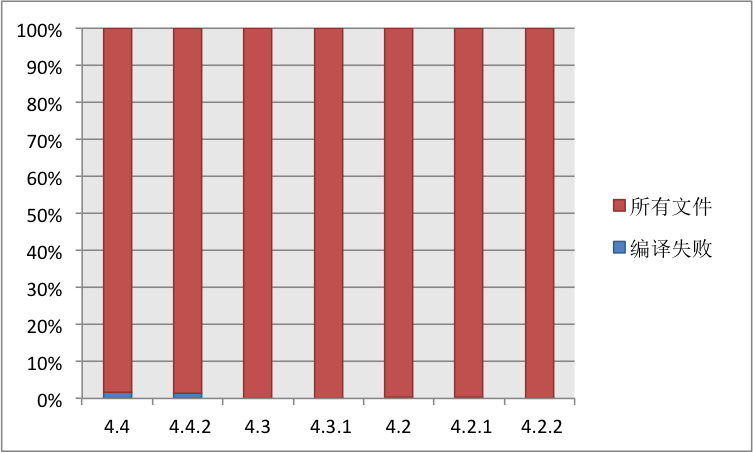
\includegraphics[width=.6\columnwidth]{merge2}
%	\caption {编译结果}
%	\label {data_compile}	
%\end{figure}

\begin{figure}[H]
	\centering
	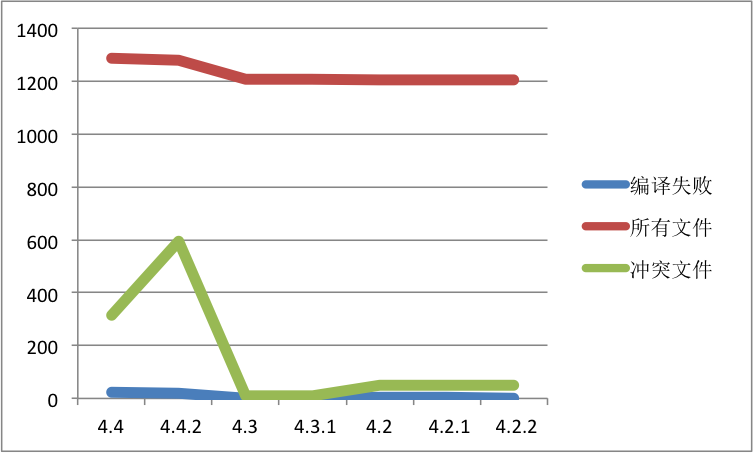
\includegraphics[width=.6\columnwidth]{merge}
	\caption {版本合并总结果}
	\label {data_merge_compile}	
\end{figure}



综上所述,本文的版本迁移过程是简单且有效的。

%在实际执行过程中,需要解决的版本合并冲突可能非常多,由于git在引导第三方工具进行冲突解决时采用的是交互式的策略,因而冲突解决需要花费较长时间和较多人力资源。为此本文采用了Apple Script撰写的脚本来辅助完成这个过程,尽可能的将其自动化。
%
%由于大部分情况下Beyond Compare提供的解决方案都是可行的,因而我们只需要采纳该解决方案即可,如果该工具无法直接提供完全正确的解决方案,则再进行人工解决即可。因而该脚本主要用于自动化实现与图形化GUI工具的交互过程,如下所述。
%
%\begin{lstlisting} [style=BashInputStyle]
%tell application "System Events"
%	repeat 300 times
%		delay 1
%		set theName to name of the first process
%			whose frontmost is true	
%		if theName is "BCompare" then		
%			delay 1	
%			keystroke "s" using {command down}	
%			delay 1	
%			if theName is "BCompare" then
%				keystroke "w" using {command down}
%			end if		
%			delay 1		
%		else
%			delay 1
%		end if
%	end repeat
%end tell
%\end{lstlisting}

\subsection{影响域分析模块}

由于整个影响域分析模块可以分为差异性分析模块和影响分析模块两个子模块,下面将分别阐述这两个子模块的实验结果并进行分析。

\subsubsection{差异性分析模块}

在差异性分析模块中,本文主要关注能够成功完成程序间语法差异性分析的文件数量。

%过滤算法的实验结果如表\ref {data_differ_1}和图\ref {differ1}所示。从结果来看,本文的过滤算法对原有的ASTro工具的直接输出结果进行了有效的过滤,有将近10\%的文件出现了伪变更,并被成功过滤。
%
%\begin{table}[H]
%	\caption{差异性分析模块结果}
%	\label{data_differ_1}
%	\centering
%	\begin{tabular}{llccc}
%		\toprule[1.5pt]
%		{\heiti 代码} & {\heiti 发行版本} & {\heiti 过滤数} & {\heiti $diff(v_2,v_1)$文件数} & {\heiti $diff(v_2,v_4)$文件数} \\\midrule[1pt]
%		Eclipse JDT Core & 4.4	& 91 & 1088 & 1172	\\		
%		Eclipse JDT Core & 4.4.2 & 94 & 1097 & 1178		\\
%		Eclipse JDT Core & 4.3 	& 110 & 1126 & 1124			\\
%		Eclipse JDT Core & 4.3.1 & 110 & 1126 & 1123			\\
%		Eclipse JDT Core & 4.2 	& 99 & 1115 & 1117		\\
%		Eclipse JDT Core & 4.2.1 & 99 & 1115 & 1116			\\
%		Eclipse JDT Core & 4.2.2 & 99 & 1115 & 1116		\\
%		\bottomrule[1.5pt]
%	\end{tabular}
%\end{table}
%
%\begin{figure}[H]
%	\centering
%	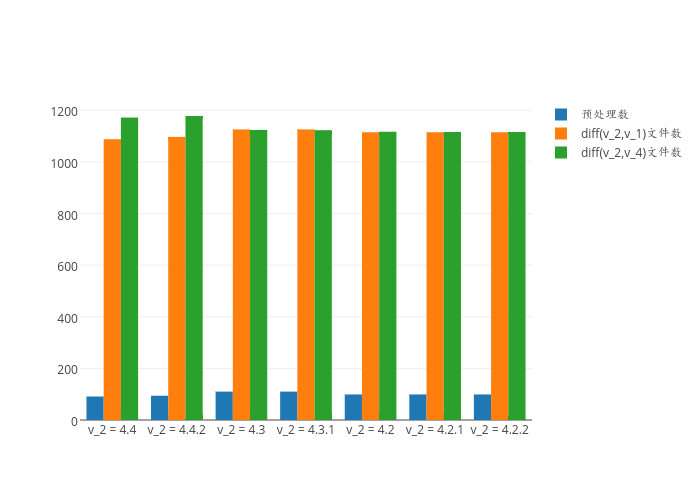
\includegraphics[width=.7\columnwidth]{differ1}
%	\caption {差异性分析模块结果}
%	\label {differ1}	
%\end{figure}
%
%
整个差异性分析模块的输出结果如表\ref {data_differ_2}和表\ref {data_differ_3}所述。更直观的表示可以参考图\ref {differ2}和\ref {differ3}。结果表明,绝大多数的文件都能够成功的进行程序间语法差异性分析,该差异性分析模块是可用的。

\begin{table}[H]
	\caption{差异性分析模块结果}
	\label{data_differ_2}
	\centering
	\begin{tabular}{llccc}
		\toprule[1.5pt]
		{\heiti $v_1$} & {\heiti $v_2$} & {\heiti $diff(v_2,v_1)$文件数} & {\heiti $v_2$文件} & {\heiti $v_1$文件} \\\midrule[1pt]
		4.3.2 & 4.4	& 1088 & 1272 & 1200\\		
		4.3.2 & 4.4.2 & 1097 & 1272	& 1200	\\
		4.3.2 & 4.3 	 & 1126 & 1200	& 1200		\\
		4.3.2 & 4.3.1  & 1126 & 1200 & 1200			\\
		4.3.2 & 4.2 	& 1115 & 1196 & 1200		\\
		4.3.2 & 4.2.1 & 1115 & 1196 & 1200		\\
		4.3.2 & 4.2.2  & 1115 & 1196 & 1200		\\
		\bottomrule[1.5pt]
	\end{tabular}
\end{table}

\begin{table}[H]
	\caption{差异性分析模块结果}
	\label{data_differ_3}
	\centering
	\begin{tabular}{llccc}
		\toprule[1.5pt]
		{\heiti $v_4$} & {\heiti $v_2$} & {\heiti $diff(v_2,v_4)$文件数} & {\heiti $v_2$文件} & {\heiti $v_4$文件} \\\midrule[1pt]
		基于4.4 & 4.4	& 1172 & 1272 &	1278\\		
		基于4.4.2 & 4.4.2 & 1178 & 1272 & 1274		\\
		基于4.3 & 4.3 	 & 1124 & 1200	& 1202		\\
		基于4.3.1 & 4.3.1  & 1123 & 1200	& 1202		\\
		基于4.2 & 4.2 	& 1117 & 1196 & 1198		\\
		基于4.2.1 & 4.2.1 & 1116 & 1196	& 1198		\\
		基于4.2.2 & 4.2.2  & 1116 & 1196 & 1198		\\
		\bottomrule[1.5pt]
	\end{tabular}
\end{table}

\begin{figure}[H]
	\centering
	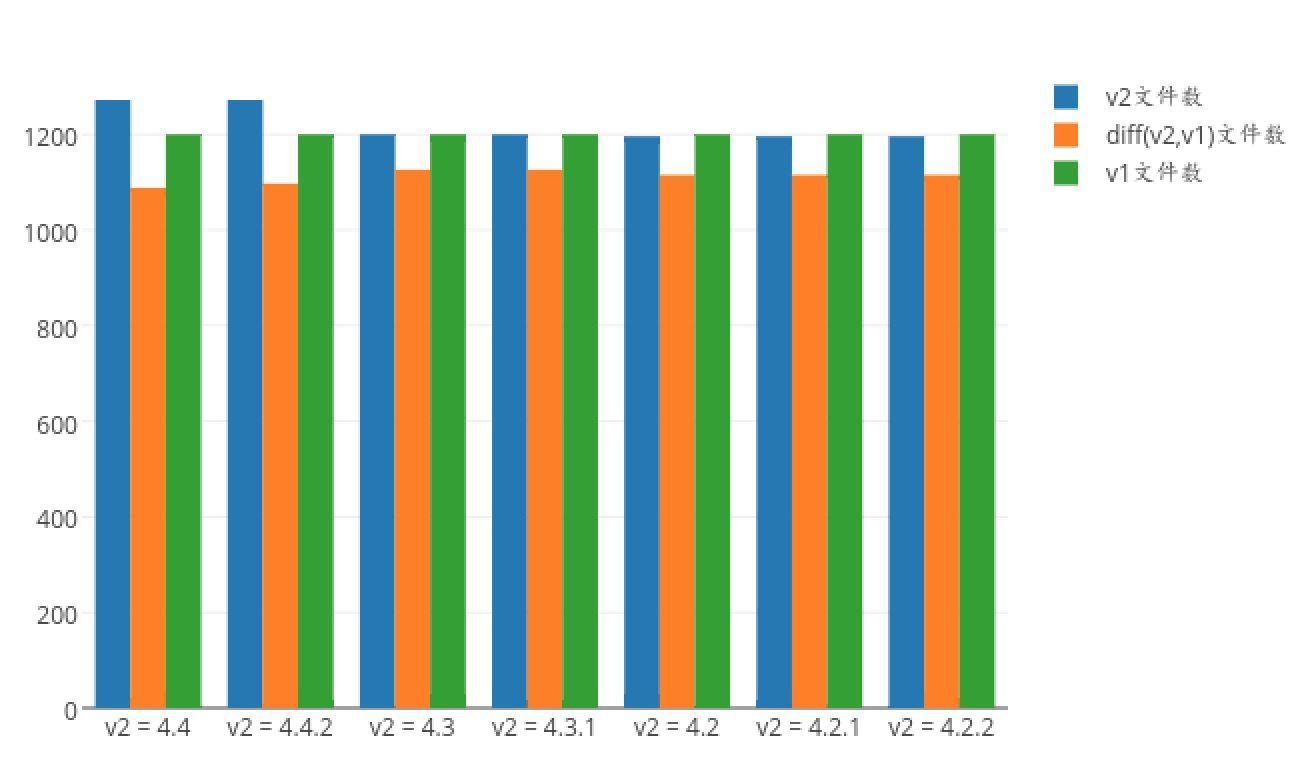
\includegraphics[width=.7\columnwidth]{differ2}
	\caption {差异性分析模块结果}
	\label {differ2}	
\end{figure}



\begin{figure}[H]
	\centering
	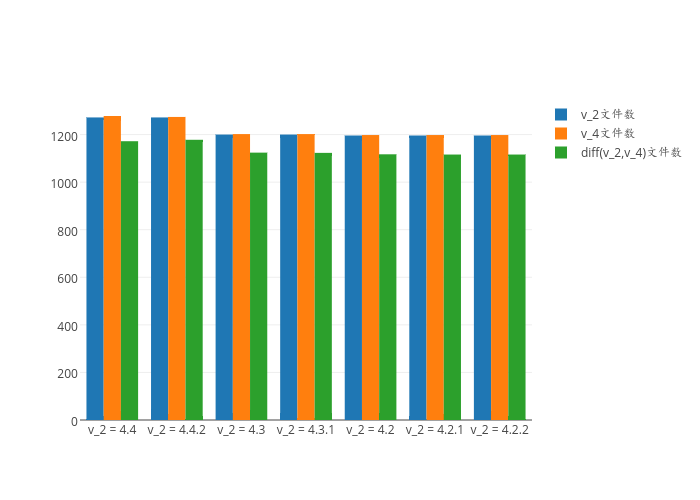
\includegraphics[width=.7\columnwidth]{differ3}
	\caption {差异性分析模块}
	\label {differ3}	
\end{figure}




\subsubsection{影响分析模块}

在影响分析模块中,本文主要关注能够成功进行分析的文件数量。

对$impact(diff(v_2,v_1),v_2)$过程而言,应用影响分析模块后,分析结果如表\ref {data_impact_1}所述。从结果中可以看出,4.3.x和4.2.x系列版本的成功分析数量略多于4.4.x系列的版本。

\begin{table}[H]
	\caption{影响分析模块结果}
	\label{data_impact_1}
	\centering
	\begin{tabular}{llcc}
		\toprule[1.5pt]
		{\heiti 代码} & {\heiti $v_2$} & {\heiti 成功分析数}  \\\midrule[1pt]
		Eclipse JDT Core & 4.4	 & 881	\\
		Eclipse JDT Core & 4.4.2 & 892 	\\
		Eclipse JDT Core & 4.3	 & 930		\\
		Eclipse JDT Core & 4.3.1 & 930 	\\
		Eclipse JDT Core & 4.2 	 &	918		\\
		Eclipse JDT Core & 4.2.1 & 923	\\
		Eclipse JDT Core & 4.2.2  & 924		\\
		\bottomrule[1.5pt]
	\end{tabular}
\end{table}

综合考虑其输入数据的数量进行对比,其结果如图\ref {impact1}所示。可以发现虽然4.4.x系列版本中代码文件的数量增加了,但其能成功分析的文件数量反而减少了。

\begin{figure}[H]
	\centering
	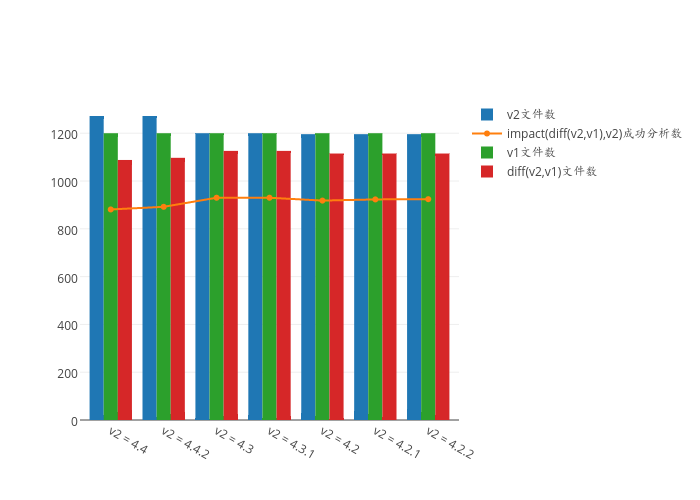
\includegraphics[width=.7\columnwidth]{impact1}
	\caption {影响分析模块}
	\label {impact1}	
\end{figure}

对$impact(diff(v_2,v_4),v_2)$过程而言,应用影响分析模块后,分析结果如表\ref {data_impact_2}所述。该过程中能够成功分析的文件数量与$impact(diff(v_2,v_1),v_2)$相类似。

\begin{table}[H]
	\caption{影响分析模块结果}
	\label{data_impact_2}
	\centering
	\begin{tabular}{llcc}
		\toprule[1.5pt]
		{\heiti 代码} & {\heiti $v_2$} & {\heiti 成功分析数}  \\\midrule[1pt]
		Eclipse JDT Core & 4.4	 & 881	\\
		Eclipse JDT Core & 4.4.2 & 892	 	\\
		Eclipse JDT Core & 4.3	 & 930			\\
		Eclipse JDT Core & 4.3.1 & 925	 	\\
		Eclipse JDT Core & 4.2 	 & 916			\\
		Eclipse JDT Core & 4.2.1 	 & 924		\\
		Eclipse JDT Core & 4.2.2 	 & 928		\\
		\bottomrule[1.5pt]
	\end{tabular}
\end{table}

综合考虑其输入数据的数量进行对比,其结果如图\ref {impact2}所示。该图中显示的成功分析的文件数量其走势与图\ref {impact1}中的结果相似。

\begin{figure}
	\centering
	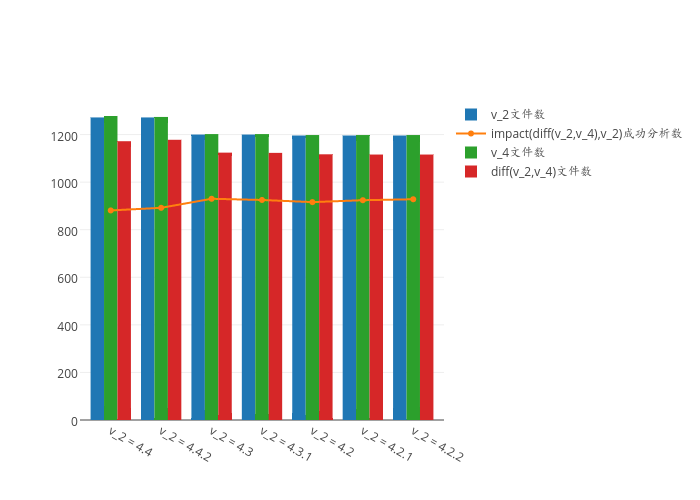
\includegraphics[width=.7\columnwidth]{impact2}
	\caption {影响分析模块}
	\label {impact2}	
\end{figure}

从结果中可以发现,大约有80\%的文件能够成功进行变更语义影响分析。无法完成分析的原因分为几种,可能是因为该文件定义了某个抽象类或接口类而没有具体实现,也可能是因为该文件没有成功完成程序间语法差异性分析过程,还可能是因为该文件编译失败而没能提供相应的源代码文件,或者可能是因为该文件确实超过了jpf-regression工具的分析能力等等。

\subsection{冲突判定模块}

在冲突判定模块中,应用本文提出的冲突检测算法后,再通过影响追踪系统进行辅助人工分析,可以得到如表\ref {data_compatible}的结果。结果表明该冲突判定模块能够找到可能发生了语义冲突的代码位置,经过人工分析,发现这些找到的代码位置确实发生了语义冲突。

\begin{table}[H]
	\caption{冲突判定结果}
	\label{data_compatible}
	\centering
	\begin{tabular}{llccc}
		\toprule[1.5pt]
		{\heiti 代码} & {\heiti $v_2$} & {\heiti 冲突文件数} & {\heiti 影响域重叠}  \\\midrule[1pt]
		Eclipse JDT Core & 4.4 	& 2 & 2 \\
		Eclipse JDT Core & 4.4.2 & 3 & 3 \\
		Eclipse JDT Core & 4.3 	& 3 & 3 \\
		Eclipse JDT Core & 4.3.1 & 3 & 3 \\
		Eclipse JDT Core & 4.2 	& 4 & 4 \\
		Eclipse JDT Core & 4.2.1 & 3  &	3 \\
		Eclipse JDT Core & 4.2.2 & 4 & 4 \\
		\bottomrule[1.5pt]
	\end{tabular}
\end{table}

%然而,在不使用过滤算法的情况下,实验结果如表\ref {data_compatible_2}所示。将表\ref {data_compatible}和表\ref {data_compatible_2}中的数据进行对比,如图\ref {conflict_data}所示,冲突判定模块确实能够找到补丁间的语义冲突。但是在不使用过滤算法时误报的影响域重叠数量陡增,这主要是差异性分析模块的误差所导致的。可见,程序间语法差异性分析算法的正确性对于后续分析过程而言极为重要,前置模块的误差会在后续模块的结果中得到显著体现。
%
%\begin{table}[H]
%	\caption{冲突判定结果}
%	\label{data_compatible_2}
%	\centering
%	\begin{tabular}{llccc}
%		\toprule[1.5pt]
%		{\heiti 代码} & {\heiti $v_2$} & {\heiti 冲突文件数} & {\heiti 影响域重叠} \\\midrule[1pt]
%		Eclipse JDT Core & 4.4 	& 2 & 59 \\
%		Eclipse JDT Core & 4.4.2 & 3 & 64 \\
%		Eclipse JDT Core & 4.3 	& 3 & 69 \\
%		Eclipse JDT Core & 4.3.1 & 3 & 66 \\
%		Eclipse JDT Core & 4.2 	& 4 & 64 \\
%		Eclipse JDT Core & 4.2.1 & 3 & 63 \\
%		Eclipse JDT Core & 4.2.2 & 4 & 65 \\
%		\bottomrule[1.5pt]
%	\end{tabular}
%\end{table}

\begin{figure}[H]
	\centering
	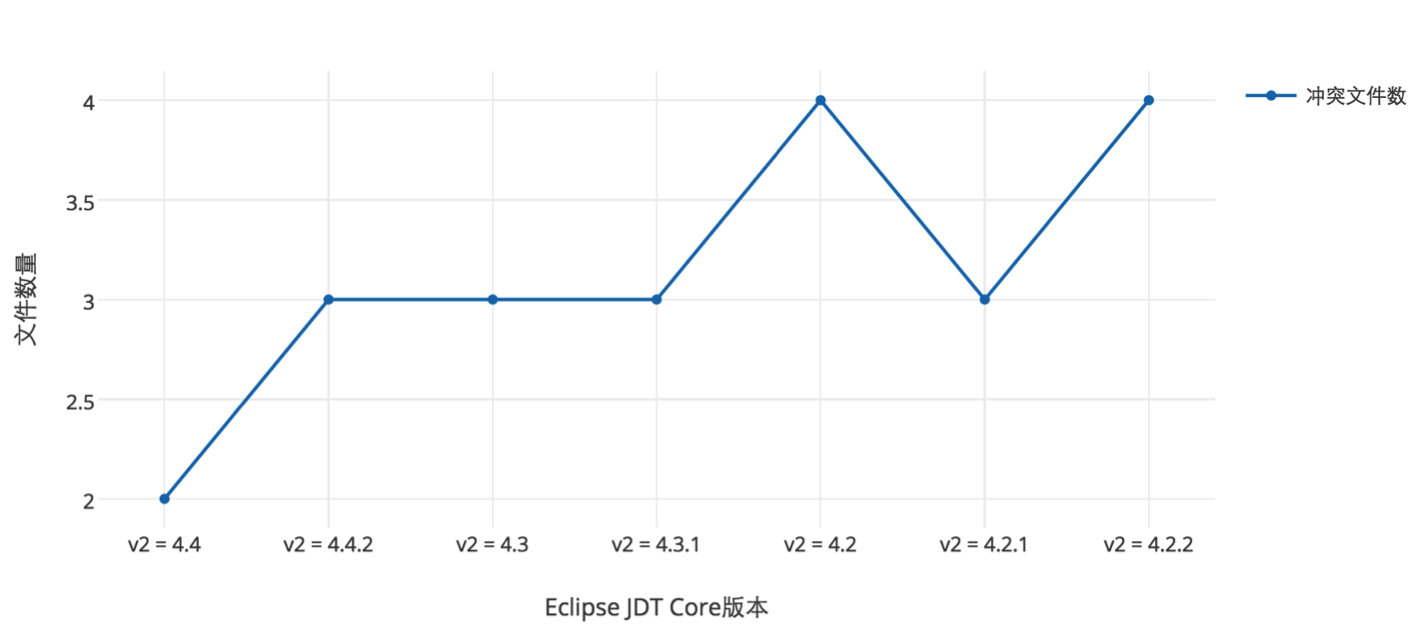
\includegraphics[width=.8\columnwidth]{conflict1}
	\caption {冲突判定模块}
	\label {conflict_data}	
\end{figure}


%
%由于运用了过滤算法,实验中找到的冲突结果都是由于针对不同语句的变更影响到了相同的语句而被挖掘出来的。事实上,如果存在修改相同语句的多个变更,其所导致的冲突在版本合并的过程中就会暴露出来。

由于前置的影响域分析模块中的变更语义影响分析算法所计算得到的是限制在变更所处方法内部的,以基本块为单位的变更影响域,因而可能会导致对冲突的漏报,这可能是造成找到的语义冲突数量较少的主要原因。

从以上结果中可以发现,本文所实现的兼容性检测工具确实能够成功分析工业界的实际项目代码,如Eclipse JDT Core(仅有少部分代码无法得出分析结果),也确实能够找到补丁间的语义冲突,这些语义冲突分散并深藏在上千个代码文件中,很难被直接发现。目前检测工具能够找到的语义冲突数量较少,这种情况可能是由于确实只有少量语义冲突存在,或者可能是由于工具的精度不够高、分析的变更影响范围不够广等因素而导致的,具体是哪种情况还有待以后做进一步的分析,虽然不排除可能出现语义冲突数量确实很少的情况,但本文认为第二种情况的可能性更高。
%\begin{itemize}
%	\item 
%	\item 
%	\item 
%	\item 
%		\begin{itemize}
%			\item 
%			\item 
%		\end{itemize}
%		
%\end{itemize}

综上所述,本文中所实现的兼容性检测工具对于工业界的实际项目而言是可用的、正确的,然而其实用性还有待进一步的提高。

\section{本章小结}
本章中主要介绍了实验的设计、实验案例的选取,并给出了实验的结果和相关分析。
章节\ref {exp_des}中主要介绍了实验的设计,包括了设计的目的以及实验的过程。
章节\ref {exp_data}中主要介绍了实验案例的选取过程。
章节\ref {exp_result}中主要介绍了实验的结果和对结果的分析。